
Voici le tableau de variations de la fonction $h$.

\begin{tikzpicture}
\tkzTabInit[lgt=1,espcl=2]{ $x$ / 1,$h $ / 2}
{ $-10$ , $-1$ ,10,20}
\tkzTabVar{-/$-5$,+/$7$,-/$-5$,+/$10$ }
\end{tikzpicture}
\begin{enumerate}
\item Comparer $h(2)$ et $h(6)$.
\item Comparer $h(-2)$ et $h(0)$.
\item Comparer $h(15)$ et $h(20)$.
\item Pour quelle valeur de $x$, $h(x)$ est maximal ? Que vaut ce maximum ?
\item Pour quelle valeur de $x$, $h(x)$ est minimal ? Que vaut ce minimum ?
\item Est-il vrai que $h(x)=-6$ admet une solution ? Justifier.
\item Est-il vrai que $h(x)=0$ admet trois solutions ? Justifier.
\end{enumerate}